\chapter{Methods}

\section{Figures}
An example is Figure~\ref{Landslide}
\begin{figure}[h] % [h] bepaalt de plaats waar de figuur komt in de tekst
    \centering % figuur komt in het midden terecht
    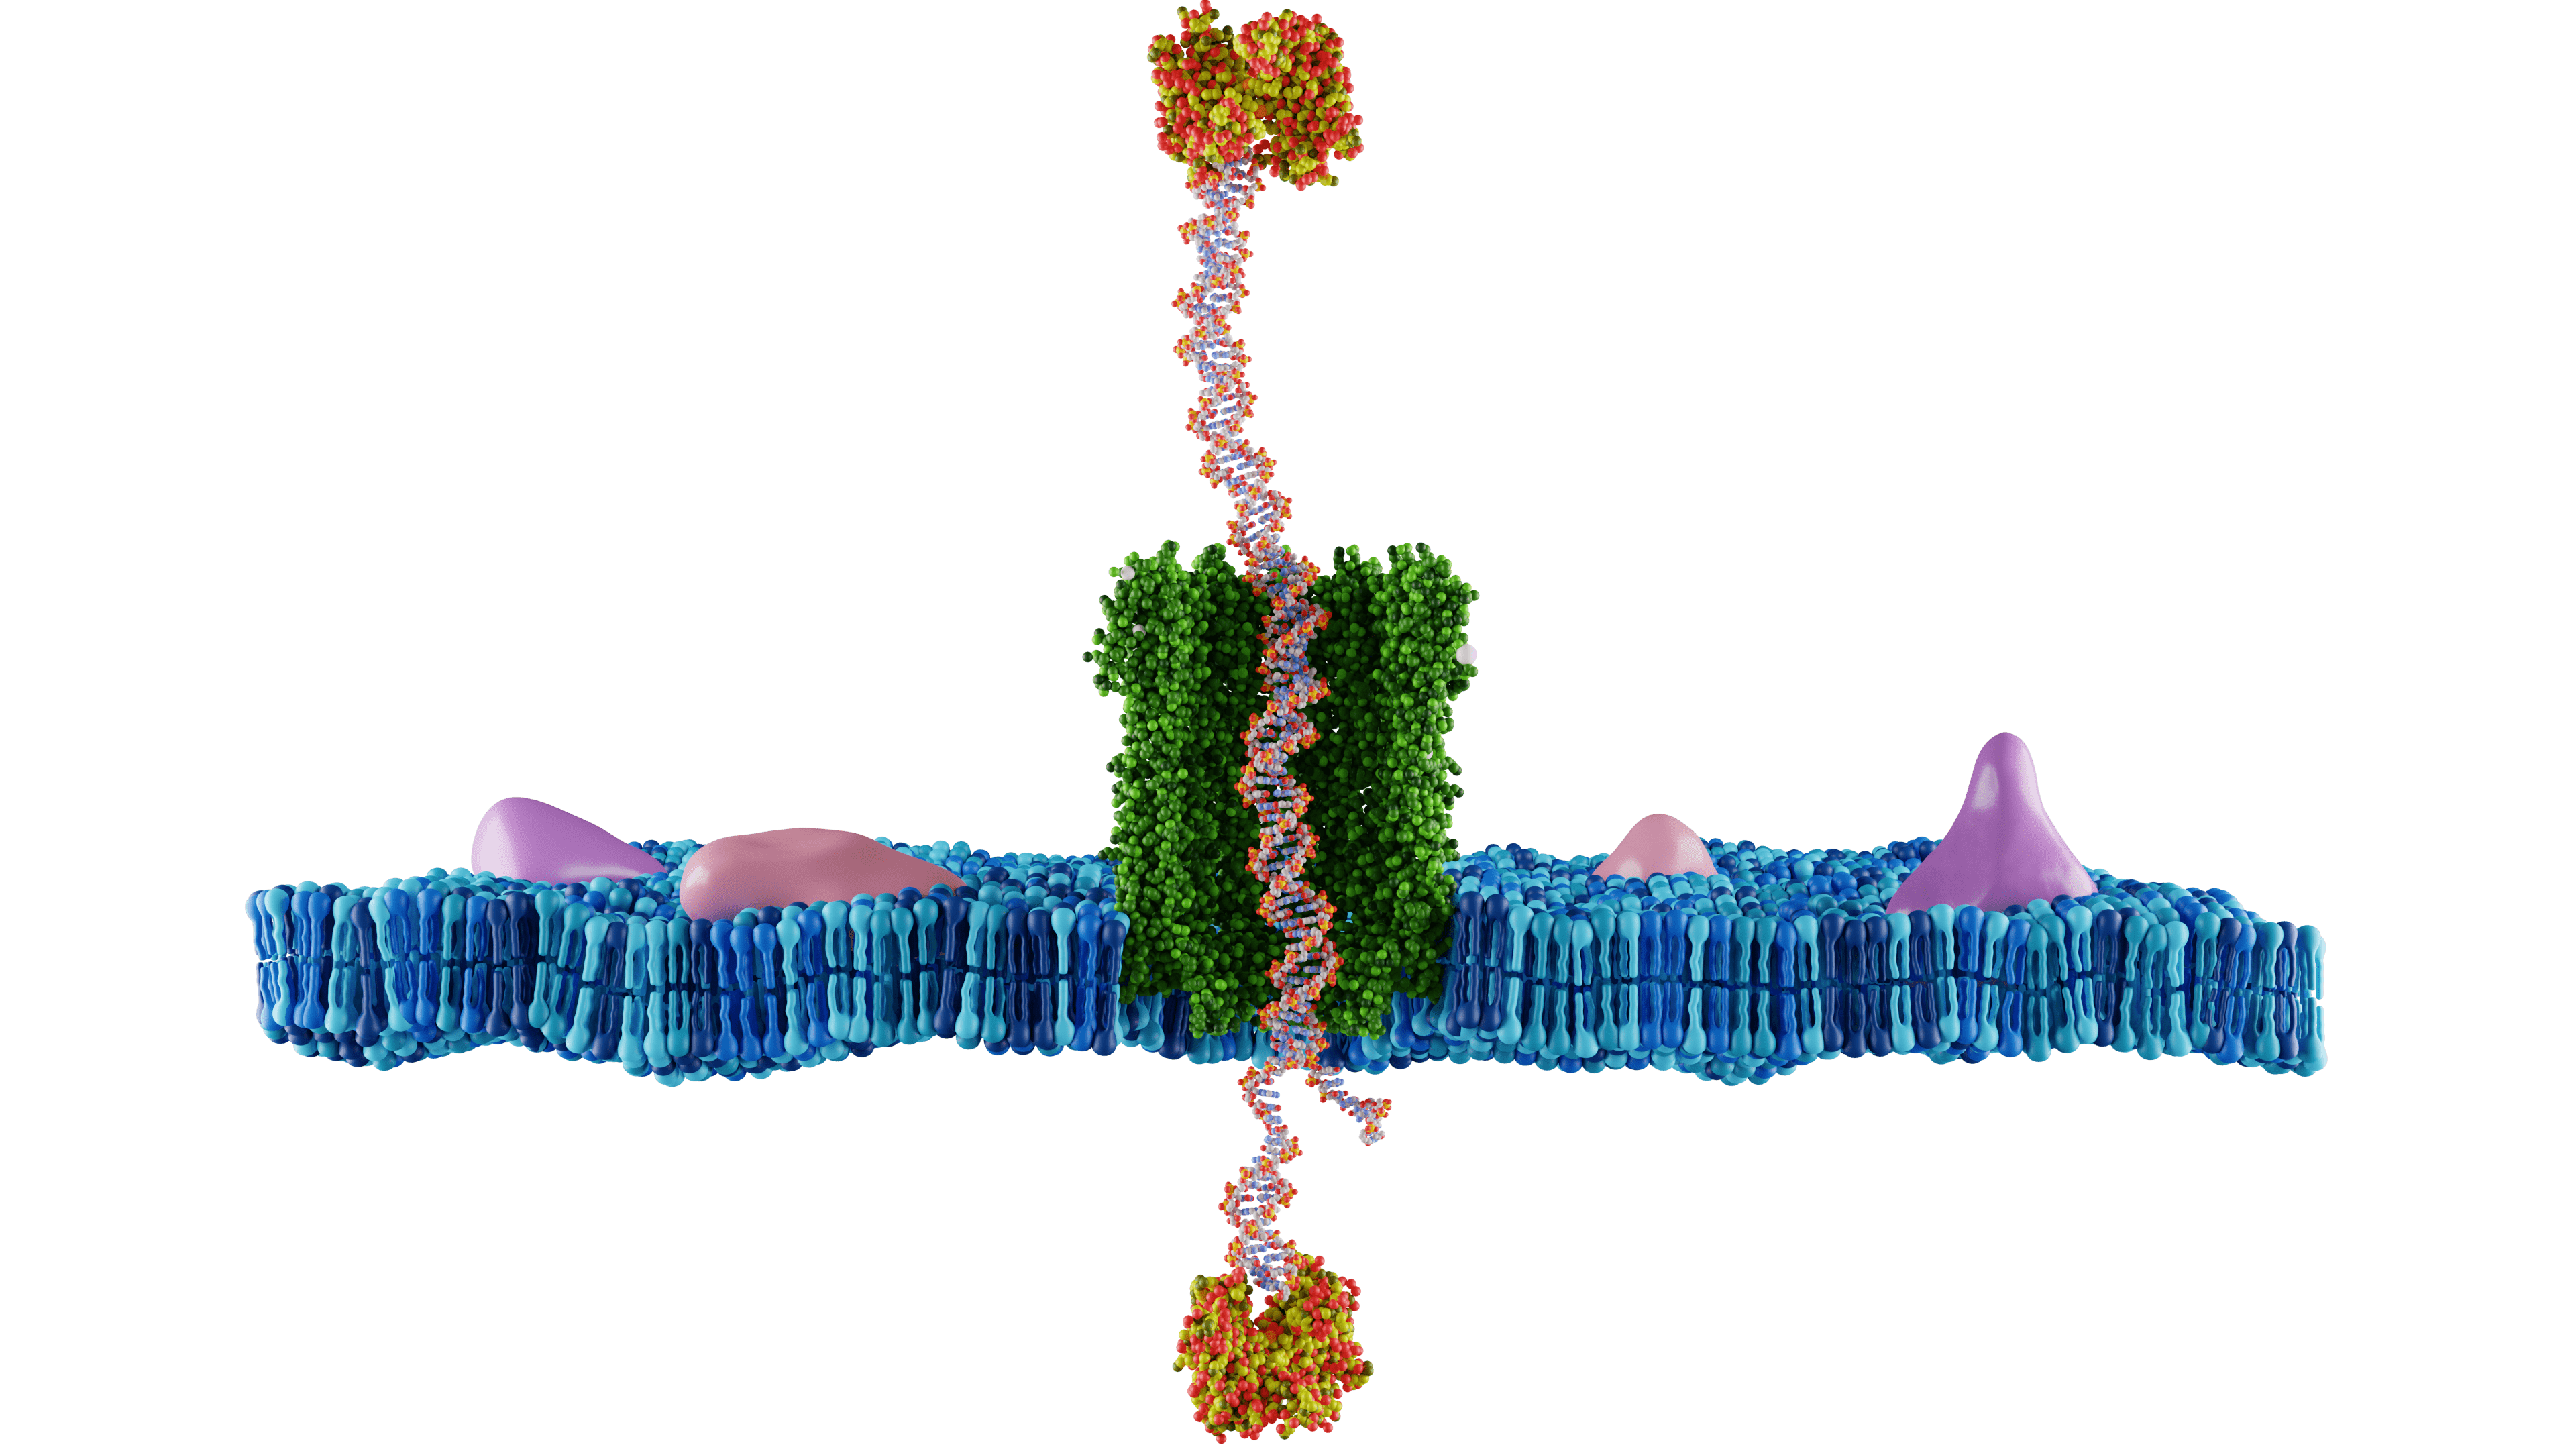
\includegraphics[width=0.8\textwidth]{Figures/CoverPhoto.png}
    \caption{A landslide.}
    \label{Landslide}
\end{figure}

\newpage

\section{Tables}
An example is Table~\ref{Tabel1}
\begin{table}[h]
    \centering
    \begin{tabular}{|c|c|}
        \hline
       Model  &  Accuracy  \\ \hline
        regression & 90\%                \\ \hline
        random forests & 95\%           \\ \hline
    \end{tabular}
    \caption{A random table.}
    \label{Tabel1}
\end{table}

\newpage

\section{Equations}
Equations can be inserted in the text itself, working in the \textit{mathmode}(put text between \$-signs, for example $Y_i=\frac{1}{x}$). Or put them in the text as a numbered floating element (e.g.\ Equation~\eqref{Eq1}).
\begin{equation}\label{Eq1}
    y=\frac{1}{x}
\end{equation}

\begin{equation}
    y=\int_{a}^{b} x^2 dx
\end{equation}

\begin{equation}
    y=\sum_{i=1}^{n} x_i^2
\end{equation}

You can align the equations:

\begin{align}
    y &=\frac{1}{x} \\
    y &=\int_{a}^{b} x^2 dx \\
    y &=\sum_{i=1}^{n} x_i^2
\end{align}
